%Please see the readme file for instructions and copy right information.
\documentclass{article}
\usepackage{csquotes}
\usepackage{graphicx}
\usepackage[margin=2.5cm]{geometry}
\newcounter{framenumber}
\setcounter{framenumber}{0}
%This command automatically prints to empty, ruled lines. I have added it under each picture for taking notes in the field. You can redefine this command according to your needs.
\newcommand{\Annotate}{\stepcounter{framenumber}[\arabic{framenumber}]
\vspace{\baselineskip}
\rule{\linewidth}{1pt}\\
\rule{\linewidth}{1pt}
\vspace{2\baselineskip}
\vfill
}
%Language options: Toggle these options to get a different language. If you add a language version, I recommend you use the same setup.
%\newcommand{\Bislama}[1]{#1}
\newcommand{\Bislama}[1]{} 
\newcommand{\English}[1]{#1}
%\newcommand{\English}[1]{}

\begin{document}
\center 
{\huge \Bislama{Bandel Banana}
	\English{Bananas in the water}

\normalsize
\Bislama{Storian ia hemi kamaot long Saliba aelan mo Logea aelan long Niu Gini.}
\English{This is a story from Saliba and Logea islands in New Guinea.}
} 
\vfill

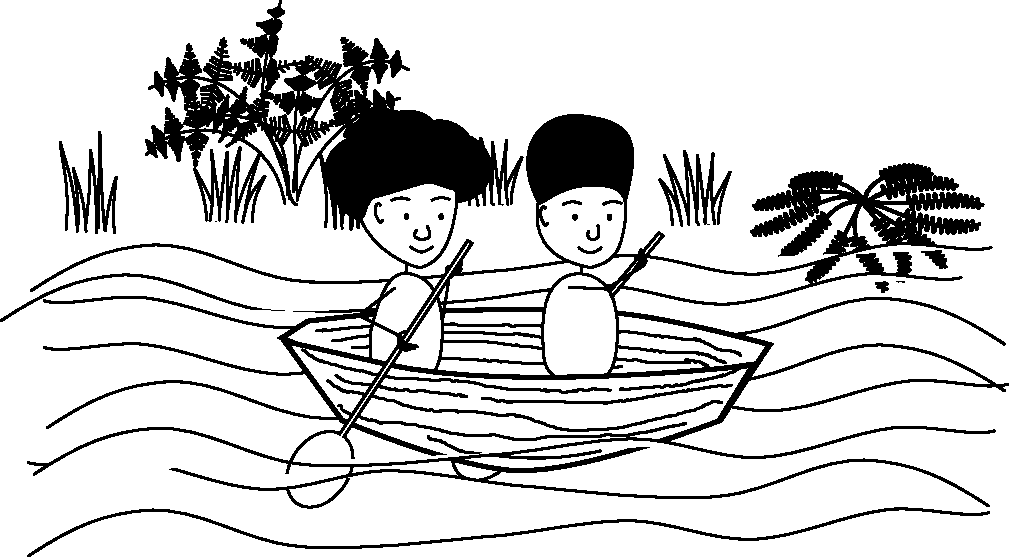
\includegraphics[scale=.7]{StoryboardBananas01}

\Bislama{Hemia Bong wetem fren blong hem, Adam. Tufala i stap rao long reva.}
\English{This is Bong and his friend, Adam. The two are rowing down the river.}

\Annotate

\pagebreak
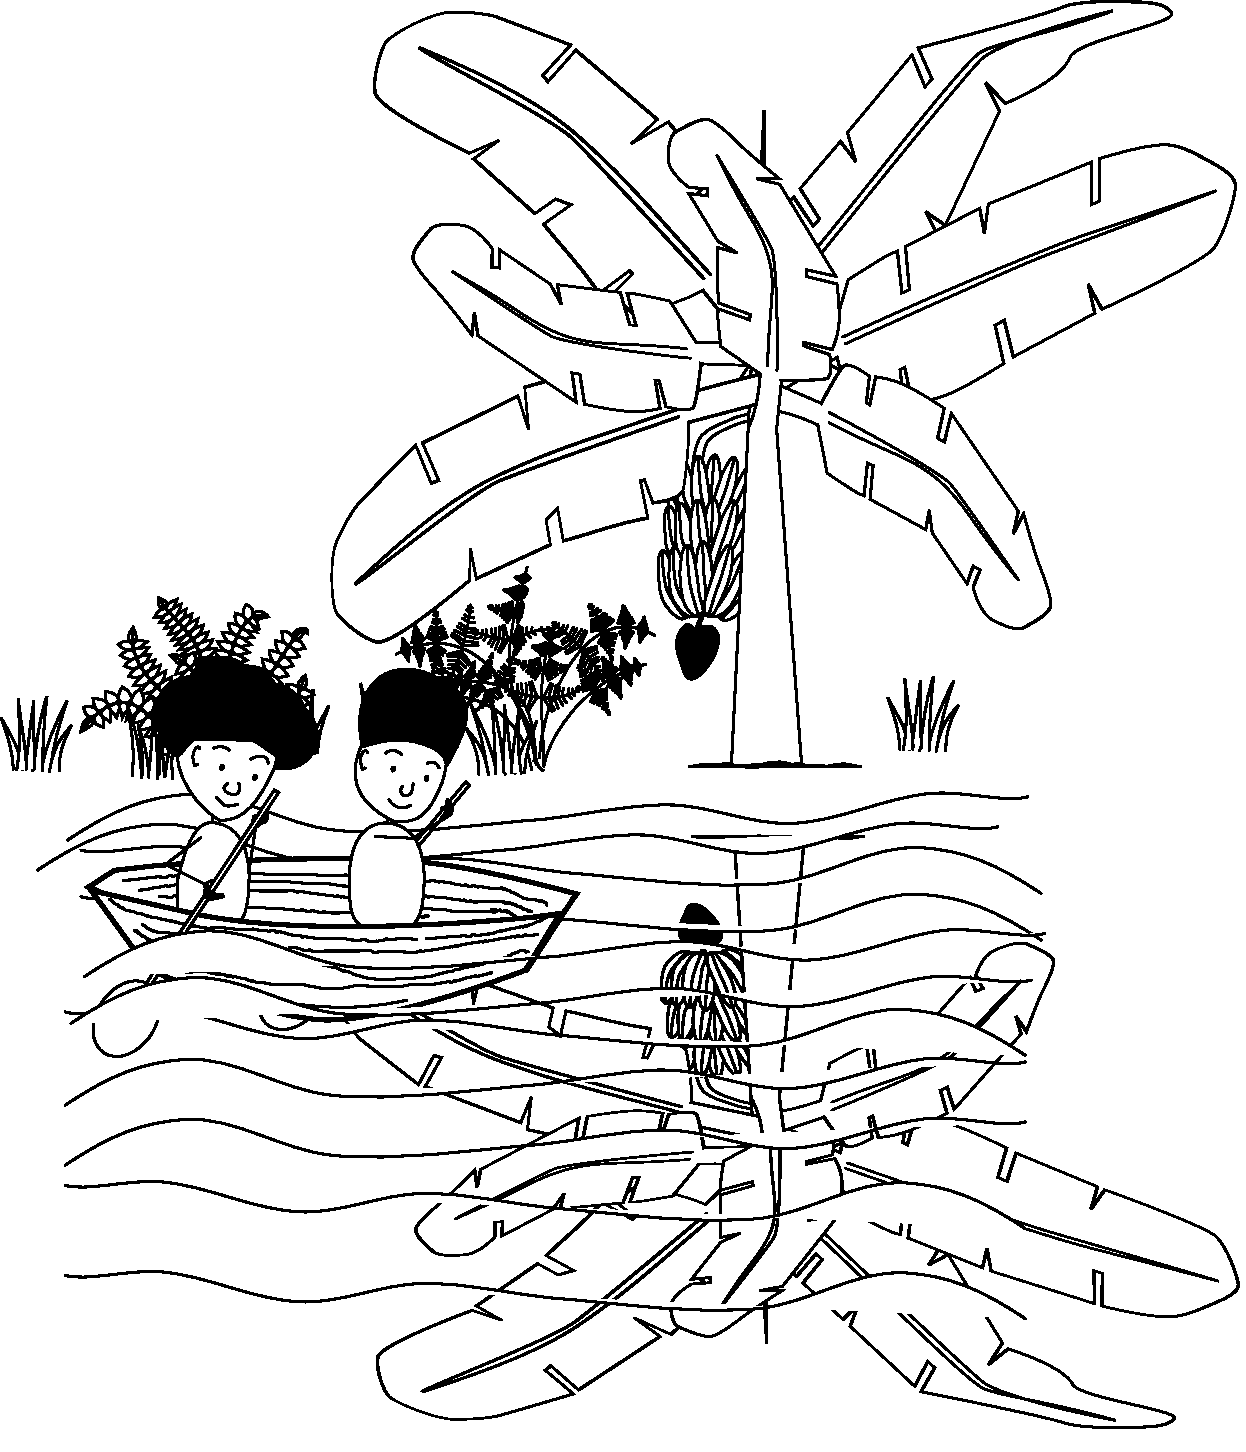
\includegraphics[scale=.6]{StoryboardBananas02}

\Bislama{Rao gogo, tufala i luk sado blong wan stampa blong banana. Tufala stap luk i go daon nomo long wota, tufala i no lukluk i go antap.}
\English{After a while, they see the reflection of a banana plant in the water. They only look at the reflection, they do not look up to the actual plant.}

\Annotate

\pagebreak

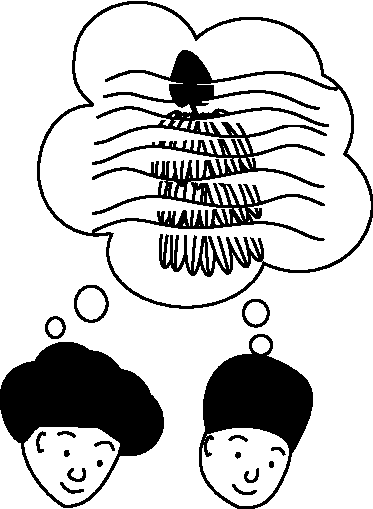
\includegraphics[scale=.7]{StoryboardBananas03}

\Bislama{Tufala i ting se bandel banana ia hemi stap long wota nomo.}
\English{The two think that the bananas are in the water.}

\Annotate

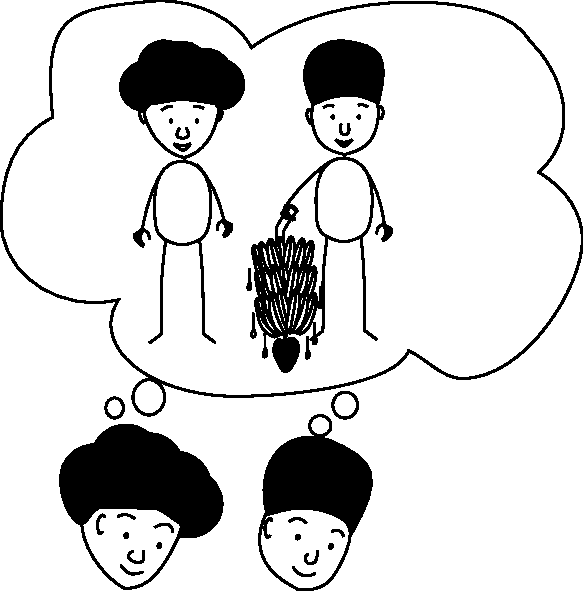
\includegraphics[scale=.6]{StoryboardBananas04.pdf}

\Bislama{Tufala i gat tingting blong stikim bandel banana ia.}
\English{They want to take the bananas out of the water.}

\Annotate

\pagebreak

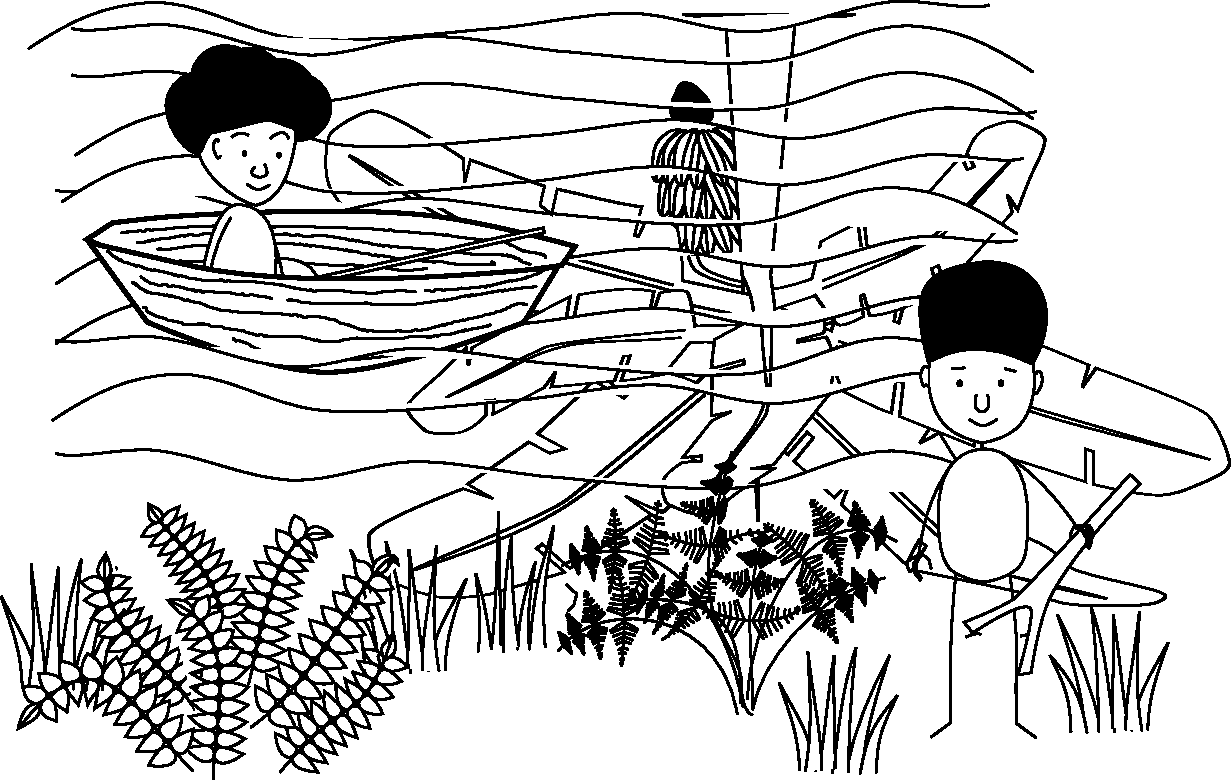
\includegraphics[scale=.6]{StoryboardBananas05.pdf}

\Bislama{Ale Adam hemi jam long soa blong karem wud blong stikim bandel banana.}
\English{So Adam goes to the shore to find a forked branch for breaking off the banana bundel.}

\Annotate

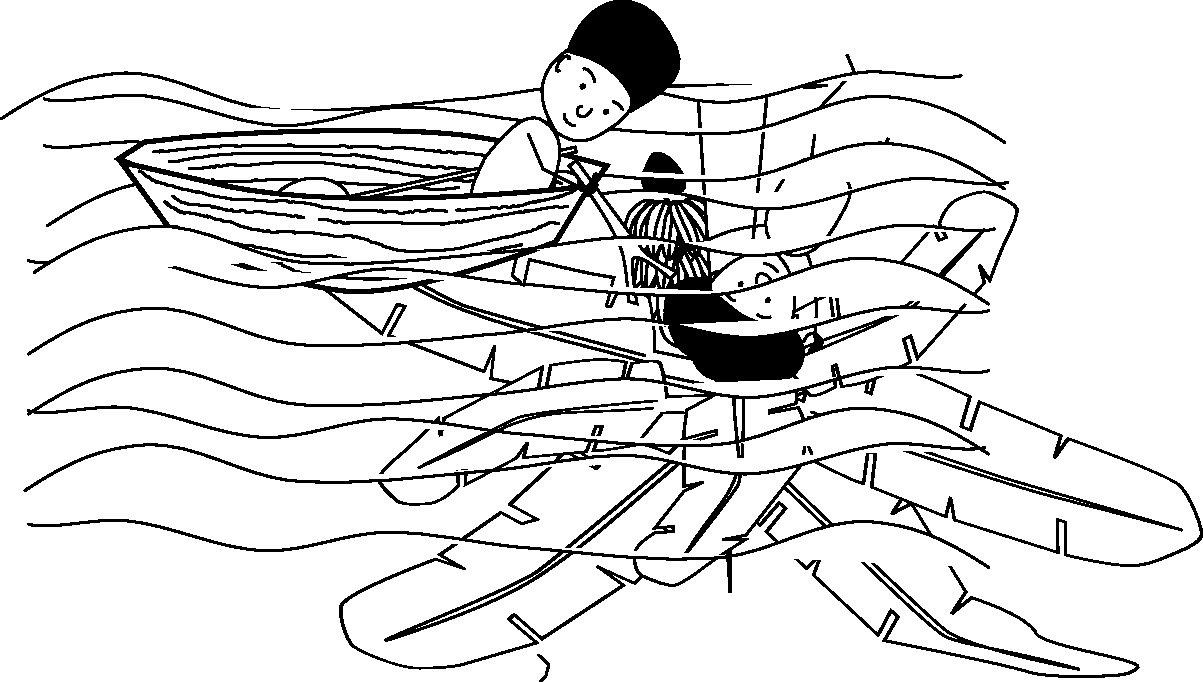
\includegraphics[scale=.6]{StoryboardBananas06.pdf}

\Bislama{Adam hemi traem stikim bandel banana, ale Bong hemi stap daeva.}
\English{Adam tries to break off the bundel with his stick while Bong is diving down to get it.}

\Annotate
\pagebreak

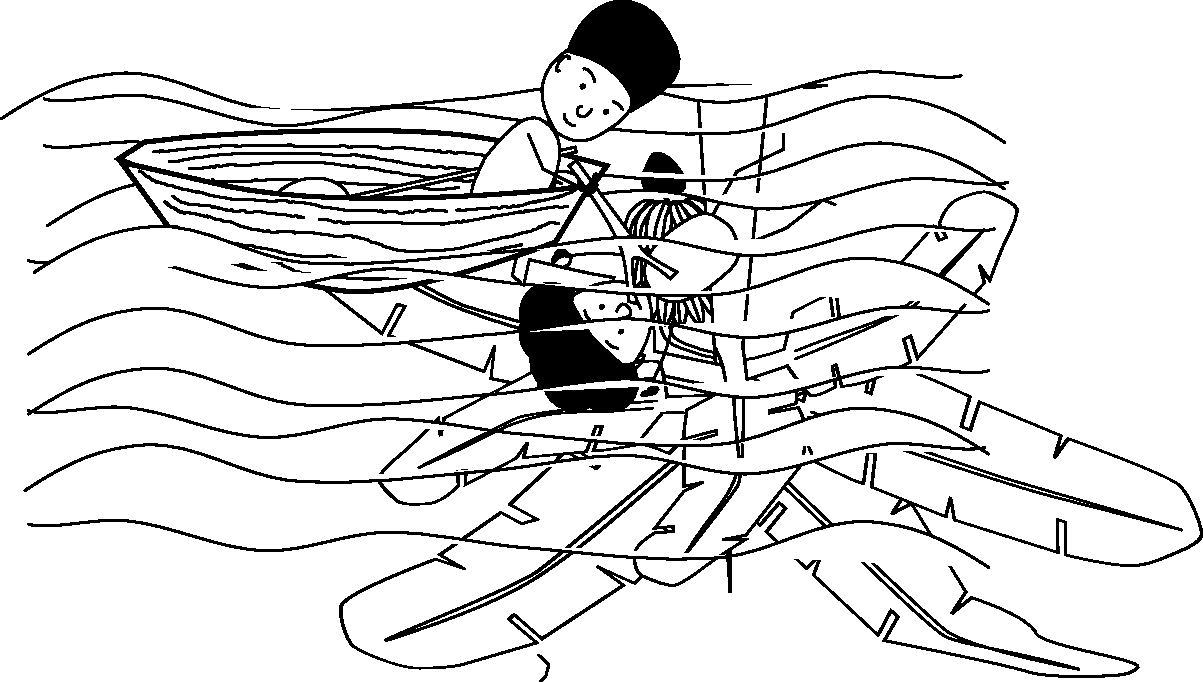
\includegraphics[scale=.6]{StoryboardBananas07.pdf}

\Bislama{Be Adam hemi no luk Bong long wota, hemi stap kilim hem long wud blong hem.}
\English{But Adam does not see his friend in the water and hits him with the stick.}

\Annotate

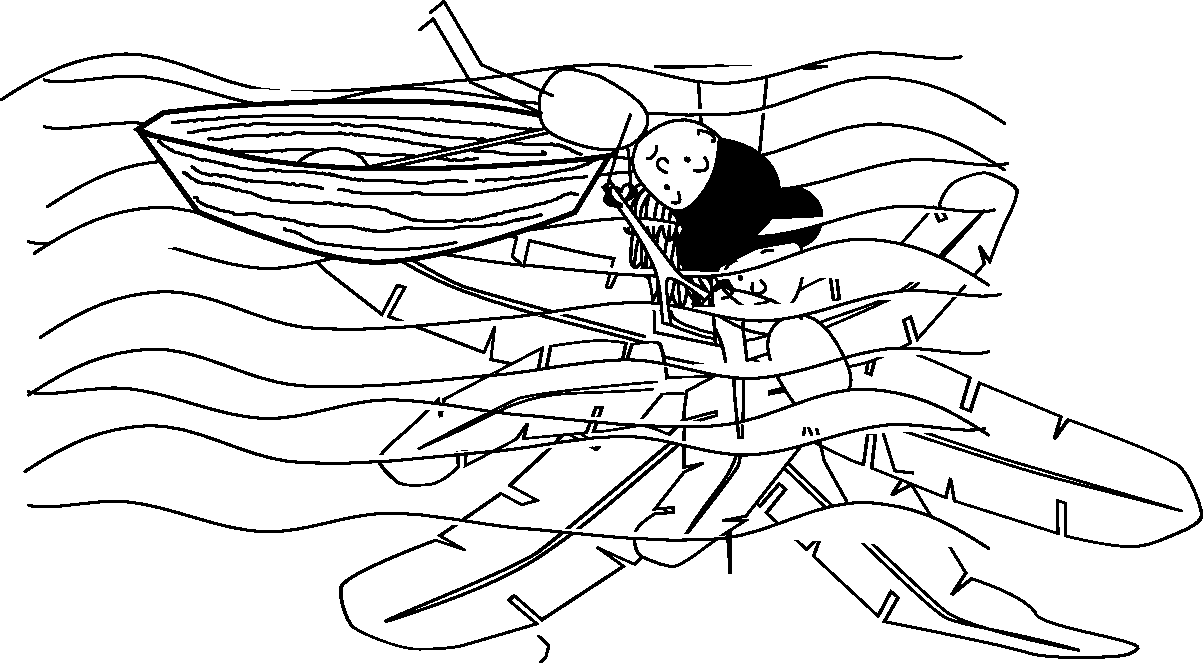
\includegraphics[scale=.6]{StoryboardBananas08.pdf}

\Bislama{Ale Bong hemi pulum wud, ale pulum Adam i go daon long wota tu.}
\English{So Bong pulls the stick and ends up pulling Adam into the water too.}

\Annotate

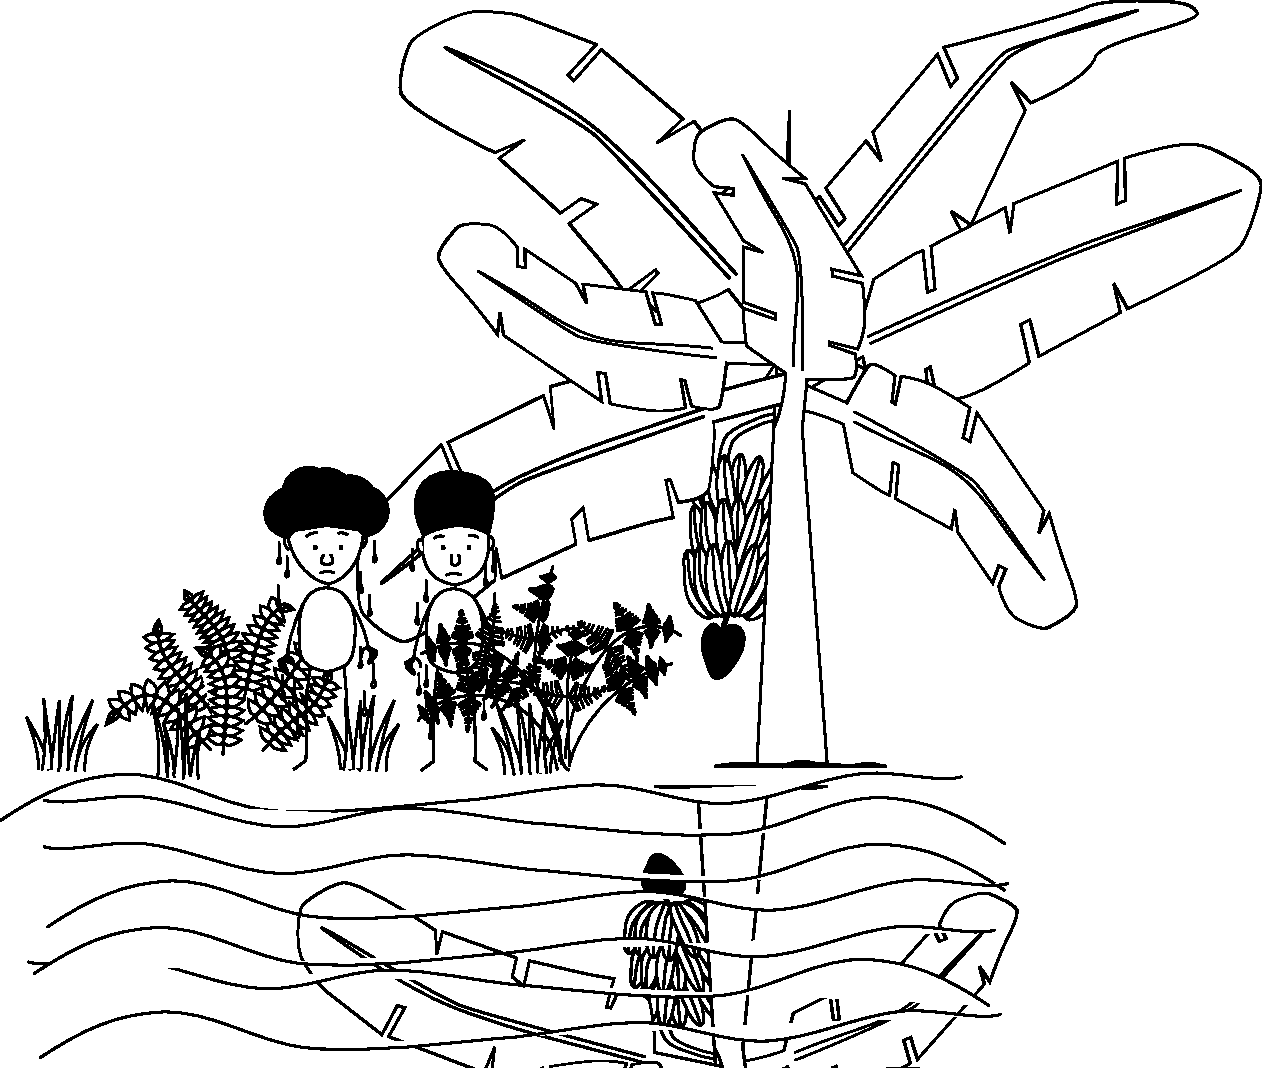
\includegraphics[scale=.45]{StoryboardBananas09.pdf}

\Bislama{Naoia we tufala i wetwet, tufala i klaem long narasaed soa.}
\English{Now that both are wet, they climb up the other side of the shore.} 

\Annotate

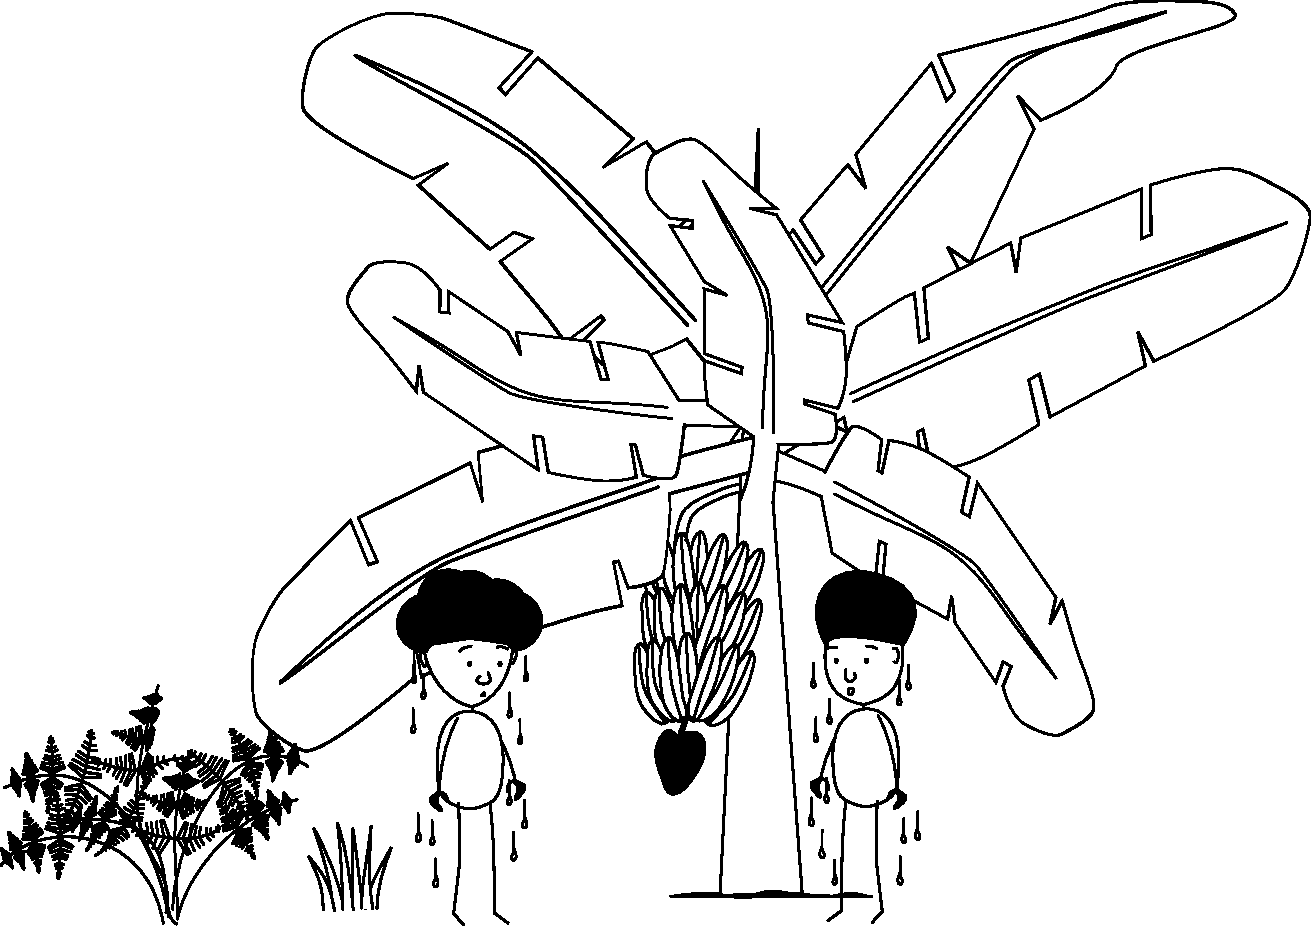
\includegraphics[scale=.45]{StoryboardBananas10.pdf}

\Bislama{Naoia nomo tufala i luk stampa blong banana long soa. Tufala i luk save se bandel we tufala i bin traem stikim hemi sado blong tru bandel ia nomo.}
\English{Only now do the two see the actual banana plant and realize their mistake.} 

\Annotate

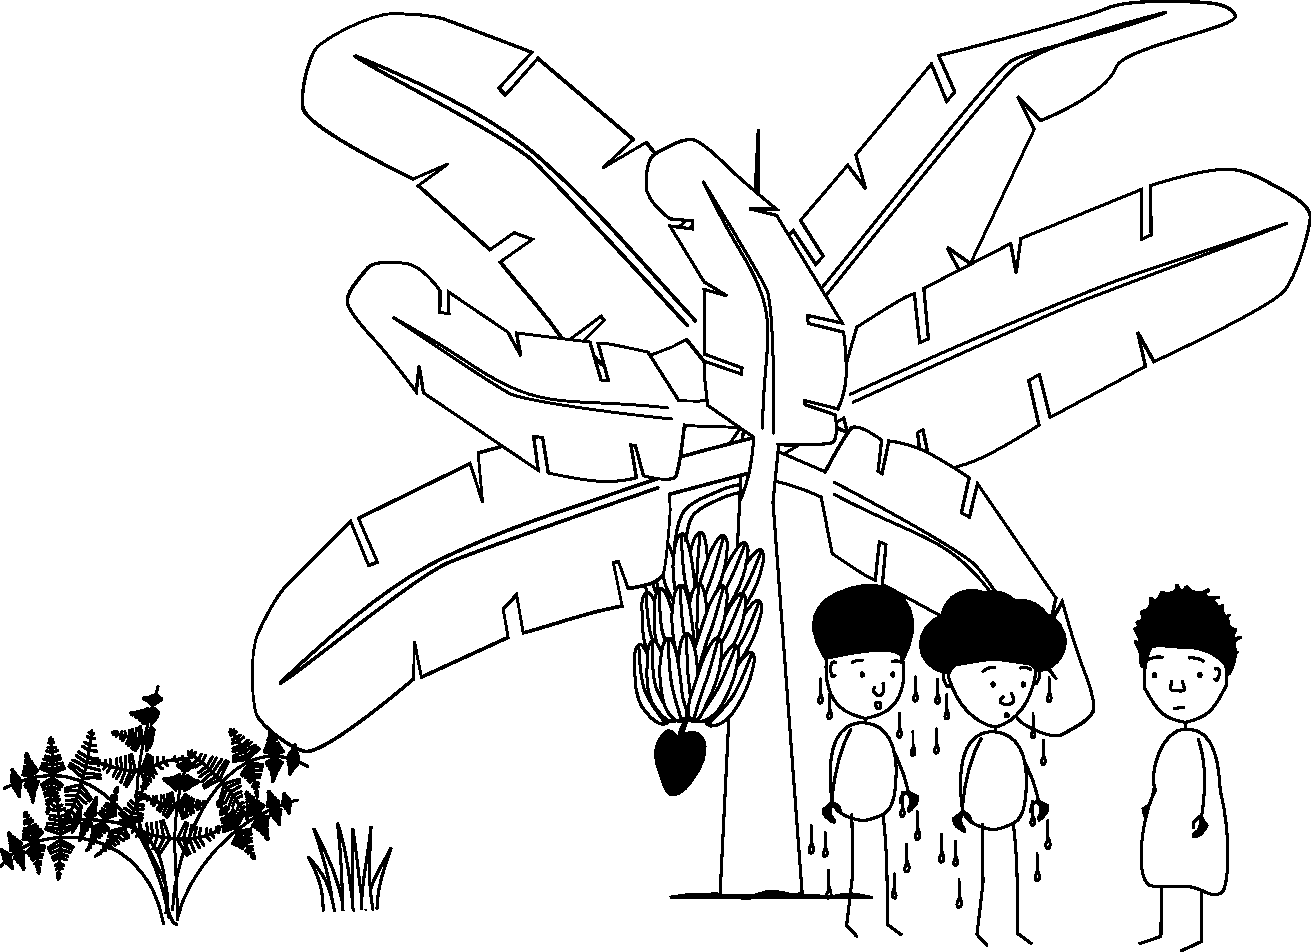
\includegraphics[scale=.5]{StoryboardBananas11.pdf}

\Bislama{Wan anti blong tufala hemi luk tufala long stampa banana ia.}
\English{An aunt of theirs sees them beside the banana plant.} 

\Annotate

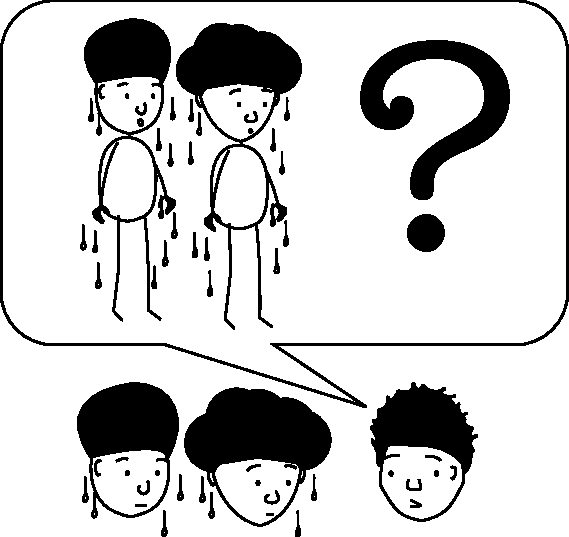
\includegraphics[scale=.6]{StoryboardBananas12.pdf}

\Bislama{Anti hemi askem tufala: \enquote{Yutufala wetwet olsem ia from wanem?}.}
\English{She asks them: \enquote{Why are you two so wet?}} 

\Annotate

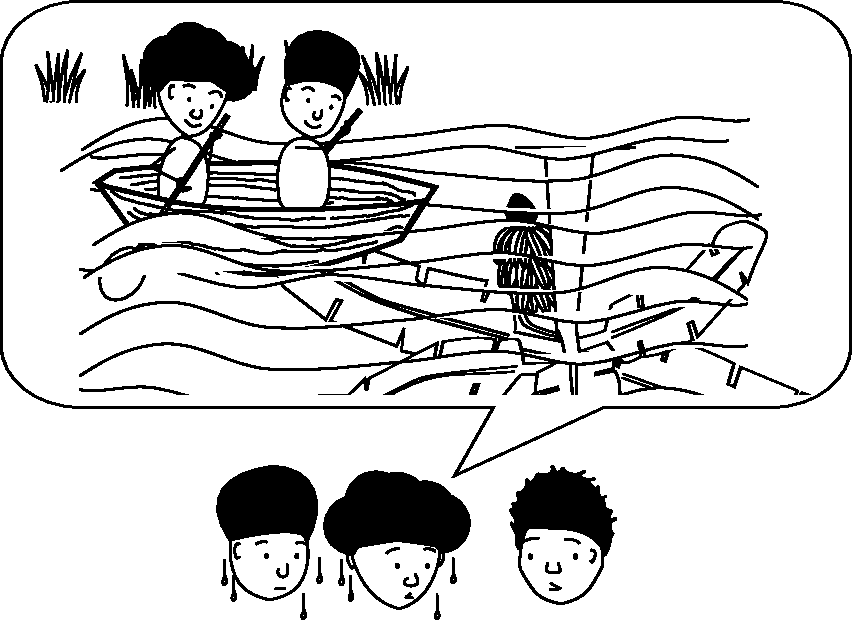
\includegraphics[scale=.6]{StoryboardBananas13.pdf}

\Bislama{Bong hemi ansa se: \enquote{Mitufala stap rao long riva, ale mitufala i lukluk sado blong wan bandel banana long wota.}}
\English{Bong says: \enquote{We were paddling along the river when we saw the reflection of bananas in the water.}} 

\Annotate


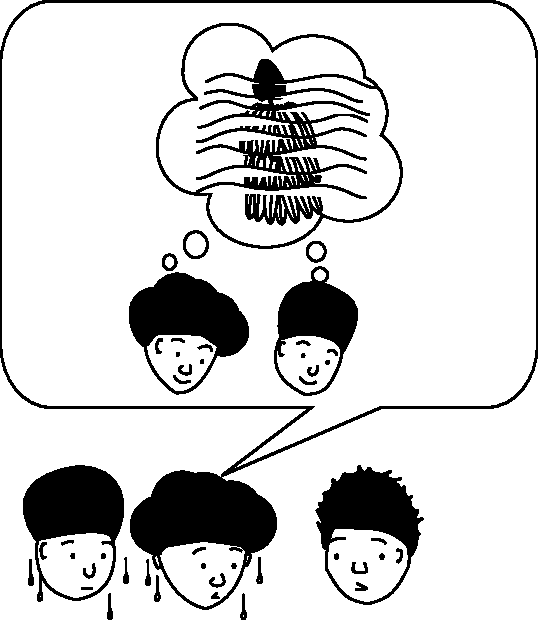
\includegraphics[scale=.6]{StoryboardBananas14.pdf}

\Bislama{Hemi se: \enquote{Mitufala i ting se bandel banana ia i stap long reva.}}
\English{Bong says: \enquote{We thought the bananas were down in the water.}} 

\Annotate
\pagebreak

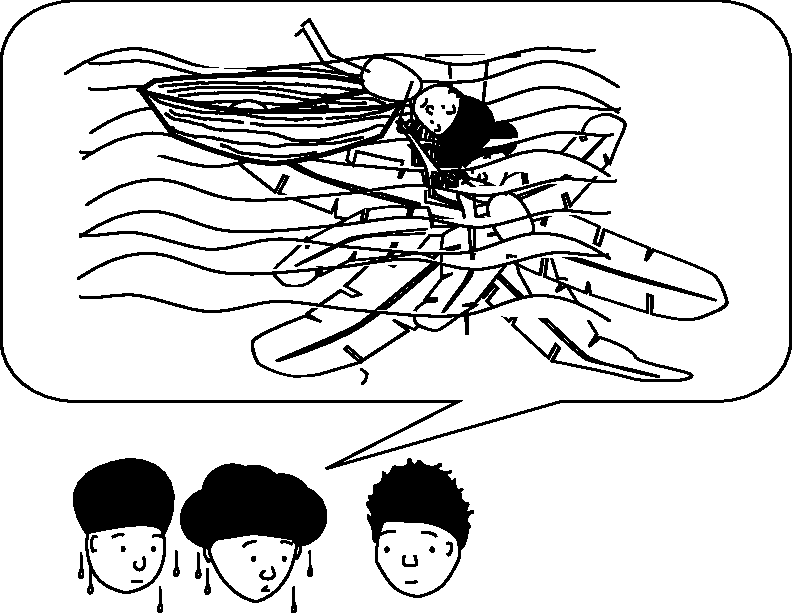
\includegraphics[scale=.6]{StoryboardBananas15.pdf}

\Bislama{\enquote{Ale, mitufala traem stikim bandel banana ia, be mitufala i fulfuldaon long wota.}}
\English{\enquote{So we tried to break off the bundel, but in the process we both ended up in the water.}} 

\Annotate

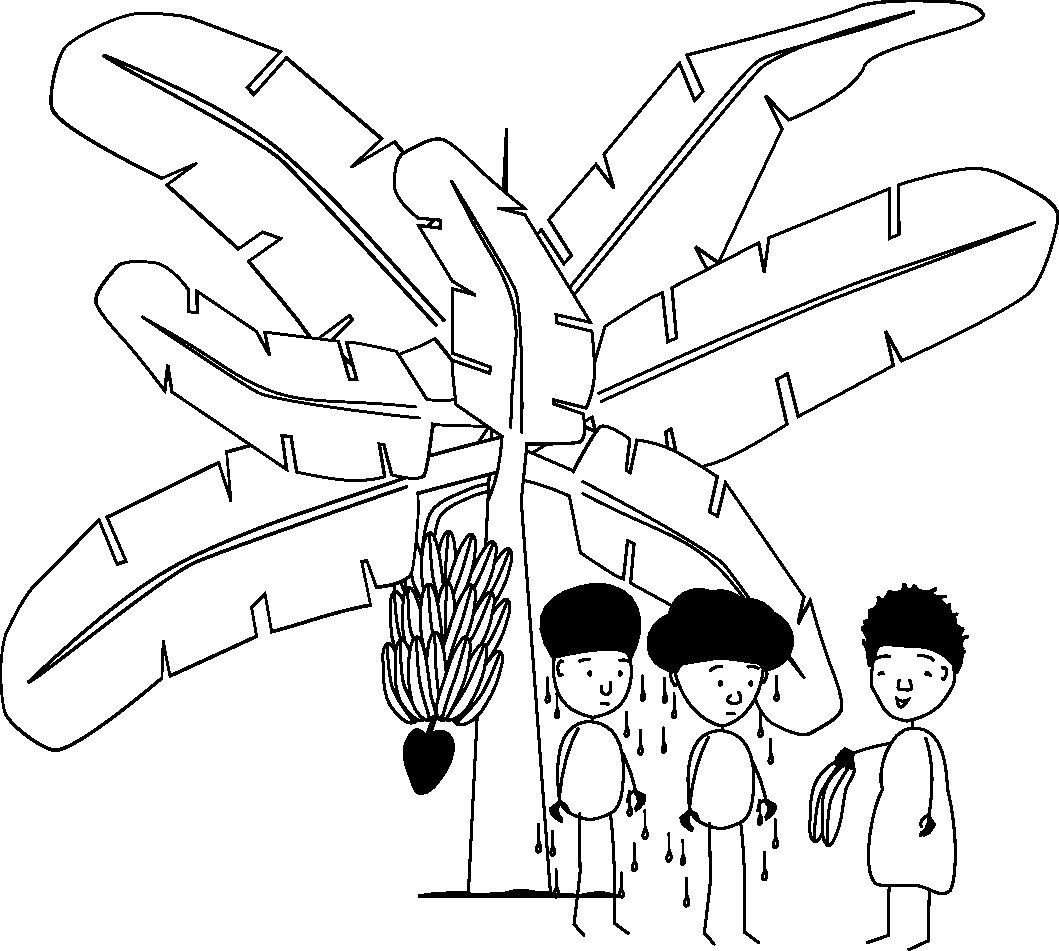
\includegraphics[scale=.6]{StoryboardBananas16.pdf}

\Bislama{Anti hemi laf nomo long kranki blong tufala boe ia. Afta hemi serem raep banana blong hem wetem tufala.}
\English{Their aunt has to laugh about their foolishness. Then she gives them a banana each to console them.} 

\Annotate


\end{document}